\documentclass[10pt]{beamer}

\usetheme{metropolis}
\usepackage{appendixnumberbeamer}

\usepackage{booktabs}
\usepackage[scale=2]{ccicons}

\usepackage{pgfplots}
\usepgfplotslibrary{dateplot}
\usepackage{verbatim}
\usepackage{fancyvrb}
\usepackage{xspace}
\newcommand{\themename}{\textbf{\textsc{metropolis}}\xspace}

\title{Status Report ALICE Computing in South Africa}
\subtitle{CHPC and University of Cape Town}
\date{\today}
\author{Sean Murray}
\institute{UCT/CHPC}
% \titlegraphic{\hfill
\includegraphics[height=1.5cm]{logo.pdf}}

\begin{document}

\maketitle

\begin{frame}{Table of contents}
  \setbeamertemplate{section in toc}[sections numbered]
  \tableofcontents[hideallsubsections]
\end{frame}



\section{Where}

\begin{frame}{ALICE in South Africa}
  \includegraphics[scale=0.25]{MonaLisaWorld.png}
\end{frame}
\begin{frame}{Cape Town Map}
  \includegraphics[scale=0.25]{CapeTown.png}
\end{frame}


\section{CHPC}
\begin{frame}{Pledges}
    \begin{tabular}
        \begin{table}{|c|c|c|}

        \end{table}
    \end{tabular}
  \begin{itemize}
  \item 600 cores for ALICE
  \item 600 cores for ATLAS
  \item 400TB each.
  \end{itemize}
\end{frame}
%

\begin{frame}{CHPC hardware}
  \begin{itemize}
      \item 6 nodes 40cores 48G RAM, dual 10GE, ce, se, se2, ui, ldap
      \item 3 nodes 40 cores, 48G RAM, quad 1GE, mon, xcat, bdii 
      \item 50 WN : dual 12core, 48 threads 196G RAM, 2x800GB of SSD.
      \item 34 WN : dual 12core, 48 threads 96GB RAM, 1 TB disk.
      \item 700+100 TB xrootd/eos
      \item 100TB Lustre
    \end{itemize}
    New main cluster on site.
    \begin{itemize}
      \item 24000 core machine seperate, in testing at the moment.
      \item 4 PB Lustre storage.
    \end{itemize}
 \end{frame}

 \begin{frame}{Grid/HEP configuration}
  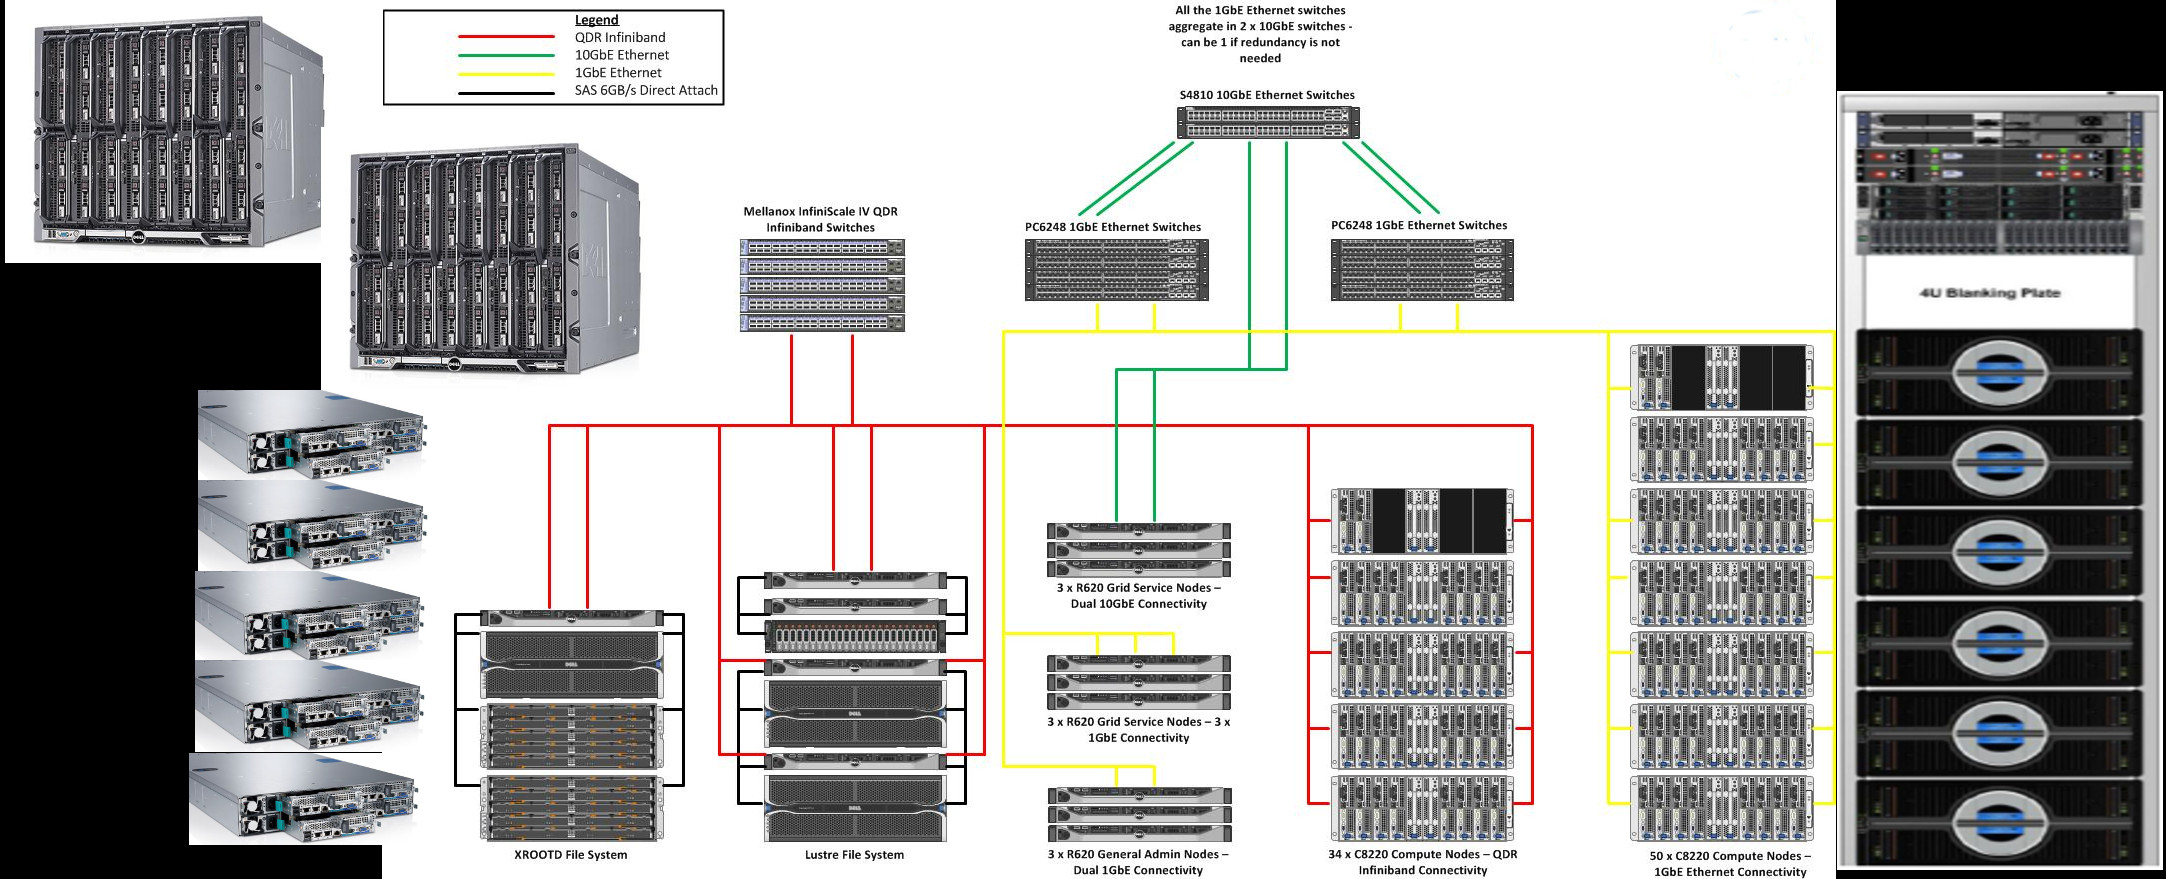
\includegraphics[scale=0.3]{CHPCConnectivityDiagram.jpg}\\
\end{frame}
\begin{frame}{Delivered Computing}
  \includegraphics[scale=0.25]{cpuonalice-4.6M.png}\\
  4.6 M hours
\end{frame}
\begin{frame}{Concurrent jobs Year}
  \includegraphics[scale=0.25]{chpcjobs-647-lastyear.png}\\
  647 average.
\end{frame}
\begin{frame}{Concurrent jobs Month}
  \includegraphics[scale=0.25]{chpcjobs-1178-lastmonth.png}\\
  1178 average.
\end{frame}


\section{Networking}
\begin{frame}{African Fibres}
  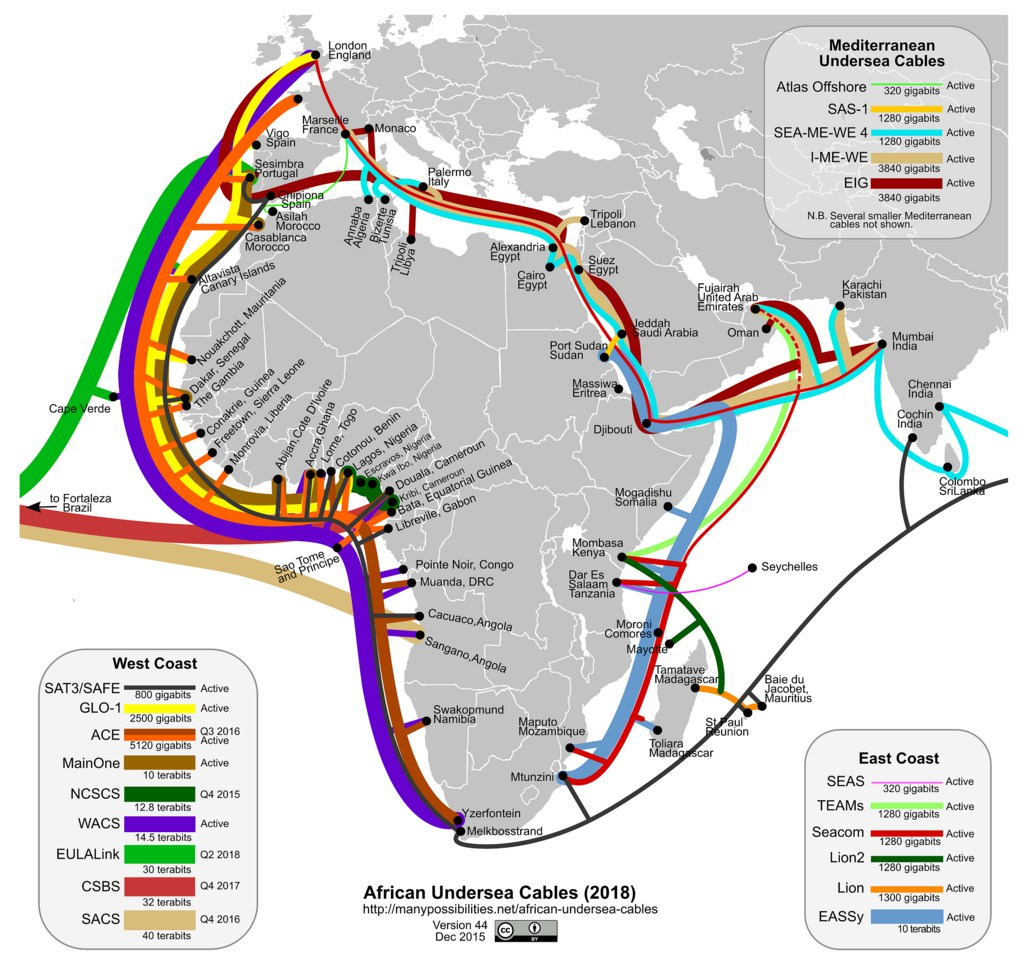
\includegraphics[scale=1]{african_undersea_cables.jpg} 
\end{frame}
\begin{frame}{African Fibres}
  \begin{itemize}
    \item WACS up west coast to Amsterdam.
    \item Seacom up east cost ending in London.
    \item CHPC 1Gbps. WACS/Seacom(failover).
  \end{itemize}
\end{frame}


\section{Monitoring}
\begin{frame}{Zabbix for all}
  \begin{itemize}
    \item monalisa client to do zabbix send of various relevant parameters.
    \item grafana for pretty pictures and dashboard.
  \end{itemize}
\end{frame}


\begin{frame}{Zabbix}
  %TODO 
    \includegraphics[scale=0.3]{ALICE-CHPC-Zabbix.png}
\end{frame}
\begin{frame}{zabbix-grafana}
  %TODO
    \includegraphics[scale=0.3]{ALICE-CHPC-Grafana.png} 
\end{frame}


\section{Disasters}
\begin{frame}{Disasters}
\begin{enumerate}
  \item Ticket renewal failure  - 25 January to ?? %TODO 
      \begin{itemize}
      \item Thursday evening switch died taking out whole cluster
      \item Network switch replaced Monday morning, so whole weekend lost.
    \end{itemize}
  \item Power issues we melted a busbar, probably been going on for a while. %TODO put in pictures.

\end{enumerate}
\end{frame}
\section{Plans}

\begin{frame}[fragile]{Plans}
  \begin{itemize}
    \item Recable the cluster.
    \item repower cluster (monitored pdu's) problem in Feb 2015
    \item new storage.
    \item HA for servers, test, building. %TODO expand with own slide.
  \end{itemize}
  {\tiny
\begin{verbatim}
EOS Console [root://localhost] |/eos/> space ls
#------------------------------------------------------------------------------------------------------------------------------------------------------------------------------------------------------
#     type #           name #  groupsize #   groupmod #N(fs) #N(fs-rw) #sum(usedbytes) #sum(capacity) #capacity(rw) #nom.capacity #quota #balancing # threshold # converter #  ntx # active #intergroup
#------------------------------------------------------------------------------------------------------------------------------------------------------------------------------------------------------
spaceview           default            0           24      4         0        156.17 M       448.02 T             0             0    off        off          20         off      2        0         off
\end{verbatim}
}
\end{frame}


\section{Ecosystem}
\begin{frame}{Eocsystem}
%TODO explain ecosystem, ska, donation, pics of stampede
\end{frame}
\begin{frame}{Questions?}
\end{frame}
%\includegraphics[scale=0.1]{FjordCruise.jpg}
\end{document}
\end{document}
